\documentclass[APA,LATO1COL]{CBNNManuscript}
\usepackage{lmodern}

\articletype{Article Type}%

\received{XXXXXX}
\revised{XXXXXX}
\accepted{XXXXXX}

\raggedbottom


\begin{document}


\title{Case-Base Neural Network: survival analysis with time-varying,
higher-order interactions}

\author[1]{Jesse Islam}

\author[2]{Maxime Turgeon}

\author[1,3]{Robert Sladek}

\author[4]{Sahir Bhatnagar}



\address[1]{\orgdiv{Department of Quantitative Life Sciences,} \orgname{McGill University}, \orgaddress{\state{Quebec}, \country{Canada}}}

\address[2]{\orgdiv{Department of Statistics}, \orgname{University of Manitoba}, \orgaddress{\state{Manitoba}, \country{Canada}}}

\address[3]{\orgdiv{Department of Human Genetics}, \orgname{McGill University}, \orgaddress{\state{Quebec}, \country{Canada}}}

\address[4]{\orgdiv{Department of Biostatistics}, \orgname{McGill University}, \orgaddress{\state{Quebec}, \country{Canada}}}

\corres{Jesse Islam \email{jesse.islam@mail.mcgill.ca}}

\presentaddress{McGill Genome Center: 740 Dr Penfield Ave, Montreal, Quebec H3A }

\abstract[Summary]{Neural network-based survival methods can model data-driven covariate interactions. While these methods can provide better predictive performance than regression-based approaches, not all can model time-varying interactions and complex baseline hazards. To address this, we propose Case-Base Neural Networks (CBNNs) as a new approach that combines the case-base sampling framework with flexible neural network architectures. Using a novel sampling scheme and data augmentation to naturally account for censoring, we construct a feed-forward neural network that may take time as an input. CBNNs predict the probability of an event occurring at a given moment to estimate the hazard function. We compare the performance of CBNNs to regression and neural network-based survival methods in a simulation and three case studies using two time-dependent metrics. First, we examine performance on a simulation involving a complex baseline hazard and time-varying interactions to assess all methods, with CBNN outperforming competitors. Then, we apply all methods to three real data applications, with CBNNs outperforming the competing models in two studies and showing similar performance in the third. Our results highlight the benefit of combining case-base sampling with deep learning to provide a simple and flexible modeling framework for data-driven, time-varying interaction modeling of single event survival outcomes. An R package is available at https://github.com/Jesse-Islam/cbnn.}

\keywords{survival analysis, machine learning, case-base, neural network}



\maketitle




\hypertarget{introduction}{%
\section{Introduction}\label{introduction}}





A common assumption in survival analysis is that the risk of the event of interest does not vary with
time (i.e. proportional hazards) \citep{hanley2009}. This simplifying assumption results in using Cox proportional
hazards models more often than smooth-in-time, accelerated failure time (AFT) models \citep{hanley2009}. This
preference causes analyses to be based on hazard ratios and relative risks rather than on survival curves and
absolute risks \citep{hanley2009}. The proportional hazards assumption in a Cox model may be incorrect in studies
where the disease pathogenesis may change over time \citep{coradini2000time}. For example, studies of breast cancer
incidence have shown that the risk of developing a tumor involves a time-varying interaction with tumor size
\citep{coradini2000time}. These time-varying covariates can be incorporated easily into AFT models \citep{royston2002flexible}.
However, these regression-based models require prior knowledge of potential
time-varying interactions and their quantitative effects.

Neural networks provide a data-driven approach to approximating interaction terms that benefit prediction. For example,
DeepSurv is a neural network-based proportional hazards model that implements the Cox partial log-likelihood
as a custom loss function \citep{katzman2018DeepSurv}. This results in a stepwise absolute risk curve that cannot
accommodate time-varying interactions. DeepSurv has shown better performance than Cox proportional hazard models in the Rotterdam and German Breast Cancer Study Group and The Molecular Taxonomy of Breast Cancer International Consortium datasets \citep{katzman2018DeepSurv}. It has also been used to develop personalized prediction models for cancers in a number of studies \citep{ds1} \citep{ds2} \citep{ds3}. Previous work suggests we may change the loss function to address
non-proportional hazards \citep{faraggi1995neural}. In contrast, DeepHit assumes an inverse Gaussian distribution
as the baseline hazard \citep{lee2018DeepHit} and specifies each follow-up time of interest in the model. DeepHit
directly estimates survival curves, rather than deriving a hazard function \citep{lee2018DeepHit}. On real datasets,
DeepHit outperformed DeepSurv \citep{lee2018DeepHit}. We note that DeepSurv and DeepHit both use custom loss
functions \citep{katzman2018DeepSurv} \citep{lee2018DeepHit}. In addition, DeepHit introduces a hyperparameter
weighing its two loss functions (negative log-likelihood and ranking losses) \citep{lee2018DeepHit}. Compared
to these neural network methods, regression-based approaches require prior specification of all interaction terms,
which makes it challenging to model covariate effects that change with time. The current neural network models
provide flexibility at the cost of clarity, while regression models provide clarity at the cost of flexibility.

We propose Case-Base Neural Networks (CBNNs) as a method for single event survival analysis that models
time-varying interactions and a flexible baseline hazard. CBNNs use the case-base sampling technique, which
allows probabilistic models to predict survival outcomes \citep{hanley2009}. After case-base sampling, we
implement a model using common neural network components that uses transformations of time as a feature
(covariate) to specify different baseline hazards. For example, by including splines of time as covariates,
case-base with logistic regression (CBLR) can approximate the Royston-Parmar flexible baseline hazard
\citep{royston2002flexible} \citep{hanley2009}. However, this still requires explicit specification of
time-varying interactions. CBNN can model both without extra tuning parameters.

In this paper, we describe the case-base sampling method and compare its properties to neural
network models, along with our hyperparameter selection procedure,
metrics and software implementation. Next, we explore the performance of CBNN, DeepSurv,
DeepHit, Cox regression and CBLR on simulated data and
describe their performance in three case studies. Finally, we explore
the implications of our results and contextualize them within neural network survival analysis in a single
event setting.




%%%%%%%%%%%%%%%%%%%%%%%%%%%%%%%%%%%%%%%%%%%%%%
%%%%%%%%%%%%%%%%%%%%%%%%%%%%%%%%%%%%%%%%%%%%%%
%%%%%%%%section2
%%%%%%%%%%%%%%%%%%%%%%%%%%%%%%%%%%%%%%%%%%%%%%
%%%%%%%%%%%%%%%%%%%%%%%%%%%%%%%%%%%%%%%%%%%%%%

\hypertarget{methods}{%
\section{Case-base neural network, metrics, hyperparameters and
software}\label{methods}}


Case-base sampling is an alternative framework for survival analysis \citep{hanley2009},
which converts the total survival time into discrete person-moments. In this section, we detail how neural
networks explicitly incorporate time as a feature while adjusting for the sampling bias in case-base
sampled data and describe the metrics and hyperparameter selection procedure used to compare
CBNN with other software packages. An R package to use CBNN is available at
\url{https://github.com/Jesse-Islam/cbnn}. The entire code base to reproduce the figures
and empirical results in this paper is available at \url{https://github.com/Jesse-Islam/cbnnManuscript}.

\hypertarget{case-base-sampling}{%
\subsection{Case-base sampling}\label{case-base-sampling}}

To implement case-base sampling, we divide the total survival time for each individual into discrete person-specific moments (person-moments) and treat each person-moment as a sample. This creates a \emph{base series} of
\emph{person-moments} where an event does not occur. This \emph{base series} complements the \emph{case series}, which contains
all person-moments at which the event of interest occurs.

For each person-moment sampled, let \(X_i\) be the corresponding covariate profile
\(\left(x_{i1},x_{i2},...,x_{ip} \right)\), \(T_i\) be the time of the person-moment and \(Y_i\) be the indicator
variable for whether the event of interest occurred at time \(T_i\). We estimate the hazard function
\(h(t \mid X_i)\) using the sampled person-moments. Recall that \(h(t \mid X_i)\) is the instantaneous
risk of experiencing the event at time \(t\) for a given set of covariates \(X_i\), assuming \(T_i \geq t\).

Now, let \(b\) be the (user-defined) size of the \emph{base series} and let \(B\) be the sum of all follow-up
times for the individuals in the study. Let $c$ be the number of events in the \emph{case series}. A
reasonable concern is determining how large $b$ should be relative to $c$, since the size of \(b\)
influences how much information is lost in the sampling process \citep{hanley2009}. The relative information when comparing two averages
is measured by $\frac{cb}{c+b}=\left[\left( \frac{1}{c}+\frac{1}{b}\right)\right]$, where $b$ is the sample size of the \emph{base series} and $c$
is the sample size of the \emph{case series}  \citep{hanley2009} \citep{mantel1}. If $b=100c$, then we expect learned weights to be at most one
percent higher than if the entire study base $B$ was used, as they are proportional to
$\frac{1}{c}+\frac{1}{100c}$ rather than $\frac{1}{c}+\frac{1}{\infty c}$ \citep{hanley2009} \citep{mantel1}.

If we sample the \emph{base series} uniformly across the study base, then the hazard function
of the sampling process is equal to \(b/B\). Therefore, we have the following equality \citep{saarela2015}
[For a rigorous treatment, see Saarela \& Hanley (2015) section 3].:
\begin{align}\label{eqn:main}
\frac{P\left(Y_i=1 \mid X_i, T_i\right)}{P\left(Y_i = 0 \mid X_i, T_i\right)} = \frac{h\left(T_i \mid X_i\right)}{b/B}.
\end{align} The odds of a person-moment being in the \emph{case
series} is the ratio of the hazard \(h(T_i \mid X_i)\) and the uniform
rate \(b/B\). Using \eqref{eqn:main}, we can see how the log-hazard
function can be estimated from the log-odds arising from case-base
sampling: \begin{align}\label{eqn:offset}
\log \left( h\left(t \mid X_i\right)\right) = \log \left(\frac{P\left(Y_i = 1 \mid X_i, t\right)}{P\left(Y_i = 0 \mid X_i, t\right)}\right) + \log\left(\frac{b}{B}\right).
\end{align}

To estimate the correct hazard function, we adjust for the bias introduced when sampling a fraction of the
study base (\(\frac{b}{B}\)) by adding the term \(\log\left(\frac{B}{b} \right)\) to offset \(\log\left(\frac{b}{B} \right)\)
during the fitting process.

\hypertarget{neural-networks-to-model-the-hazard-function}{%
\subsection{Neural networks to model the hazard
function}\label{neural-networks-to-model-the-hazard-function}}

After case-base sampling, we pass all features, including time, into any user-defined feed-forward
component (Figure \ref{fig:NNarch}). Then, we add an offset term and pass the output through a sigmoid activation function
(Figure \ref{fig:NNarch}). Since we are interested in predicting the odds of an event occurring, the sigmoid
activation function is ideal as it is the inverse of the odds and can be used to calculate the hazard. The
general form for the neural network using CBNN is:

\begin{align*}
P\left(Y=1|X,T\right)&=\mathrm{sigmoid}\left(f_{\theta}(X, T) + \log\left(\frac{B}{b}\right) \right),
\end{align*}

where \(T\) is a random variable representing the event time, \(X\) is the random variable for a covariate
profile, \(f_{\theta}(X, T)\) represents any feed-forward neural network architecture, \(\log\left(\frac{B}{b}\right)\)
is the offset term to adjust for the bias (\(\log\left(\frac{b}{B}\right)\)) set by case-base sampling, \(\theta\) is the
set of parameters learned by the neural network and \(\mathrm{sigmoid}(x)=\frac{1}{1+e^{-x}}\). By approximating
a higher-order polynomial of time using a neural network, the baseline hazard specification is now data-driven,
while user-defined hyperparameters such as regularization, number of layers and nodes control the flexibility
of the hazard function.


\begin{figure}

{\centering \includegraphics[width=1\linewidth]{../figures/Figure1.pdf}}

\caption{Methodological steps involved in CBNN. The first step, case-base sampling, is completed before training begins.
Then, we pass this sampled data through a feed-forward neural network and add an offset to adjust for the bias inherent in
case-base sampling and apply a sigmoid activation function to create a probability. Once the neural network model
completes its training, we can convert the probability output to a hazard for the survival outcome of interest.}\label{fig:NNarch}
\end{figure}


The following derivation shows how our probability estimate is converted
to odds: \begin{align*}
 \log\left( h(t \mid X) \right) &= \log\left(\frac{\mathrm{sigmoid}\left(f_{\theta}(X, T) + \log\left(\frac{B}{b}\right)\right)}{1-\mathrm{sigmoid}\left(f_{\theta}(X, T) + \log\left(\frac{B}{b}\right)\right)}\right) + \log\left(\frac{b}{B}\right) \\
 &= \log\left( \frac{\frac{\exp\left(f_{\theta}(X, T) + \log\left(\frac{B}{b}\right)\right)}{\exp\left(f_{\theta}(X, T) + \log\left(\frac{B}{b}\right)\right)+1}}{1-\frac{\exp\left(f_{\theta}(X, T) + \log\left(\frac{B}{b}\right)\right)}{\exp\left(f_{\theta}(X, T) + \log\left(\frac{B}{b}\right)\right)+1}}\right) + \log\left(\frac{b}{B}\right) \\
 &= \log\left(\exp\left( f_{\theta}(X, T) + \log\left(\frac{B}{b}\right) \right) \right) + \log\left(\frac{b}{B}\right) \\
 &= f_{\theta}(X, T) + \log\left(\frac{B}{b}\right) + \log\left(\frac{b}{B}\right) \\
&= f_{\theta}(X, T). 
\end{align*}

We use binary cross-entropy as our loss function \citep{gulli2017}:
\begin{align*}
L(\theta)=-\frac{1}{N} \sum^{N}_{i=1} y_{i} \cdot \log(\hat{f}_{\theta}(x_{i}, t_{i}) ) + (1-y_{i} )\cdot \log(1-\hat{f}_{\theta}(x_{i}, t_{i}) ),
\end{align*} where \(\hat{f}_{\theta}(x_{i}, t_{i})\) is our estimate
for a given covariate profile and time, \(y_{i}\) is our target value specifying whether an event occurred and \(N\) represents
the number of individuals in our training set.

Backpropagation with an appropriate minimization algorithm (such as Adam, RMSPropagation, stochastic gradient
descent) is used to optimize the parameters in the model \citep{gulli2017}. For our analysis, we use Adam as implemented
in Keras \citep{gulli2017}. While the size of the \emph{case series} is fixed as the number of events; the size of the
\emph{base series} is not restricted. We use a ratio of 100:1 \emph{base series} to \emph{case series} \citep{hanley2009}.
After fitting our model, we
convert the output to a hazard. To use CBNN for predictions, we manually set the offset term $\left(\log\left(\frac{B}{b} \right)\right)$
to 0 in the new data as we already account for the sampling bias during the fitting process.

Since we are directly modeling the hazard, we can readily estimate the
risk function (\(F\)) at time \(t\) for a covariate profile \(X\),
\begin{align}\label{eqn:ci2}
F\left(t\mid X\right)& = 1 - \exp\left(-\int_{0}^{t}h(u|X) \,\textrm du\right).
\end{align} We use a finite Riemann sum \citep{hughes2020calculus} to
approximate the integral in \eqref{eqn:ci2}.



\hypertarget{performance-metrics}{%
\subsection{Performance metrics}\label{performance-metrics}}

To choose our method-specific hyperparameters, we use the Integrated Brier Score (IBS) \citep{graf1999}, which is based on the
Brier Score (BS) and provides a summarized assessment of performance for each model. We assess the performance of models on
a held out dataset using two metrics: 1) the Index of Prediction Accuracy (IPA) \citep{kattan2018index}; and 2) the Inverse probability
censoring weights-adjusted time dependent area under the receiver operating characteristic curve ($AUC_{IPCW}$) \citep{auc}. The
IPA score is a metric for both discrimination and calibration, while the $AUC_{IPCW}$ provides a metric for discrimination only.

\hypertarget{bs}{%
\subsubsection{Brier Score (BS)}\label{bs}}
The BS \citep{graf1999} is defined as \begin{align}\label{eqn:bs}
BS(t)=\frac{1}{N}\sum^{N}_{i=1}\left(\frac{\left(1 - \widehat{F}(t \mid X_{i})\right)^{2}\cdot I(T_{i}\leq t,\delta_{i}=1)}{\widehat{G}(T_{i})} + \frac{\widehat{F}(t\mid X_{i})^{2}\cdot I(T_{i}>t)}{\widehat{G}(t)}\right),
\end{align} where \(\delta_{i}=1\) shows individuals who have experienced the event, \(N\) represents the number of samples
in our dataset over which we calculate \(BS(t)\), \(T_{i}\) is the survival or censoring time of an individual, \(\widehat{G}(t)=P[c>t]\) is a non-parametric estimate of the censoring distribution and \(c\) is censoring time. The BS provides a score that accounts for the
information loss because of censoring. Once we fix our \(t\) of interest, the individuals in the dataset can be divided into three
groups. Individuals who experienced the event before \(t\) are present in the first term of the equation. The second term of the
equation includes individuals who experience the event or are censored after \(t\). Those censored before \(t\) (the remaining
individuals) are accounted for by the IPCW adjustment (\(G(\cdot)\)) present on both terms.


\hypertarget{integrated-brier-score-ibs}{%
\subsubsection{Integrated Brier Score (IBS)}\label{integrated-brier-score-ibs}}

The Integrated Brier Score (IBS) is a function of the BS (\ref{eqn:bs}) \citep{graf1999}, which is defined as \begin{align*}
IBS(t)=\int_{t}^{t_{max}}BS(t)dw(t),
\end{align*} where $w(t)=\frac{t}{t_{max}}$ and $t_{max}$ is the upper bound for the survival times of interest. As the IBS is calculated for a range of follow-up-times,
it is a useful metric to track overall performance across all of follow-up time during cross-validation. We use the
IPA score to get an estimate of performance at each follow-up time for our studies.



\hypertarget{index-of-prediction-accuracy-ipa}{%
\subsubsection{Index of prediction accuracy (IPA)}\label{index-of-prediction-accuracy-ipa}}

The IPA is a function of time, based on the BS. The IPA score is given by \begin{align}
\textrm{IPA}(t) &= 1-\frac{BS_{model}(t)}{BS_{null}(t)}, \nonumber
\end{align} where \(BS_{model}(t)\) represents the BS over time \(t\) for the model of interest and \(BS_{null}(t)\) represents
the BS if we use an unadjusted Kaplan-Meier (KM) curve as the prediction for all observations \citep{kattan2018index}. The
IPA score has an upper bound of one, where positive values show an increase in performance over the null model and
negative values show that the null model performs better. As an extension of BS, the IPA score assesses both model calibration
and discrimination and show how performance changes over follow-up time \citep{graf1999} \citep{kattan2018index}.




\hypertarget{auc}{%
\subsubsection{Inverse probability censoring weights-adjusted time dependent area under the receiver operating characteristic curve ($AUC_{IPCW}$) }\label{auc}}

The IPCW-adjusted AUC ($AUC_{IPCW}$) is a time-dependent metric that considers censoring \citep{auc}. For a given follow-up time of interest,
 \begin{align*}
AUC_{IPCW}(t)=\frac{\sum^{n}_{i=1}\sum^{n}_{j=1} I \left(\widehat{F}(t|X_{i})>\widehat{F}(t|X_{j})\right) \cdot I(T_{i}\leq t,\delta_{i}=1) \cdot \left( 1-I(T_{j}\leq t,\delta_{j}=1) \right) \cdot W_{i}(t) \cdot W_{j}(t)} { \sum^{n}_{i=1}\sum^{n}_{j=1} I(T_{i}\leq t,\delta_{i}=1) \cdot \left( 1-I(T_{j}\leq t,\delta_{j}=1) \right) \cdot W_{i}(t) \cdot W_{j}(t) },
\end{align*}where \begin{align*}
W_{i}(t)=\frac{I(T_{i}\leq t,\delta_{i}=1)}{\widehat{G}(T_{i})} +\frac{I(T_{i}>t)}{\widehat{G}(t)}.
\end{align*} The $AUC_{IPCW}$ measures discrimination \citep{auc}. By examining both IPA and $AUC_{IPCW}$,
we can better understand whether a model performs better in terms of calibration or discrimination.

\hypertarget{hyperparameter-selection}{%
\subsection{Hyperparameter selection}\label{hyperparameter-selection}}

Neural networks require external parameters that constrain the learning process (hyperparameters). We apply the following hyperparameter
optimization procedure to each method for each study. First, we fix a test set with 15\% of the data which we keep aside during hyperparameter selection.
To determine the best hyperparameters for each neural network method, we use a three-fold cross-validated grid search \citep{gulli2017} on the remaining
data (85\% training, 15\% validation) for the following range of hyperparameters:
\[
Grid\ search: \begin{cases}
Learning\ rate \sim \{0.001, 0.01\} \\ 
Dropout \sim \{0.01,0.05, 0.1\} \\
First\ layer\ nodes \sim \{50, 75, 100\} \\
Second\ layer\ nodes \sim \{10,25,50\} \\
Number\ of\ batches \sim \{100, 500\} \\
Activation\ function \sim \{ReLU, Linear\}\\
\alpha \sim \{0, 0.5, 1\}. \ (DeepHit \ only)
\end{cases}
\] 

\begin{table}
\caption{Hyperparameters selected after three-fold cross-validated grid search along with the average IBS for each neural network model in the
complex simulation (A); multiple myeloma (MM) case study (B); free light chain (FLC) case study (C); and prostate cancer (Prostate) case study (D).}
\label{tab:wins}
\begin{center}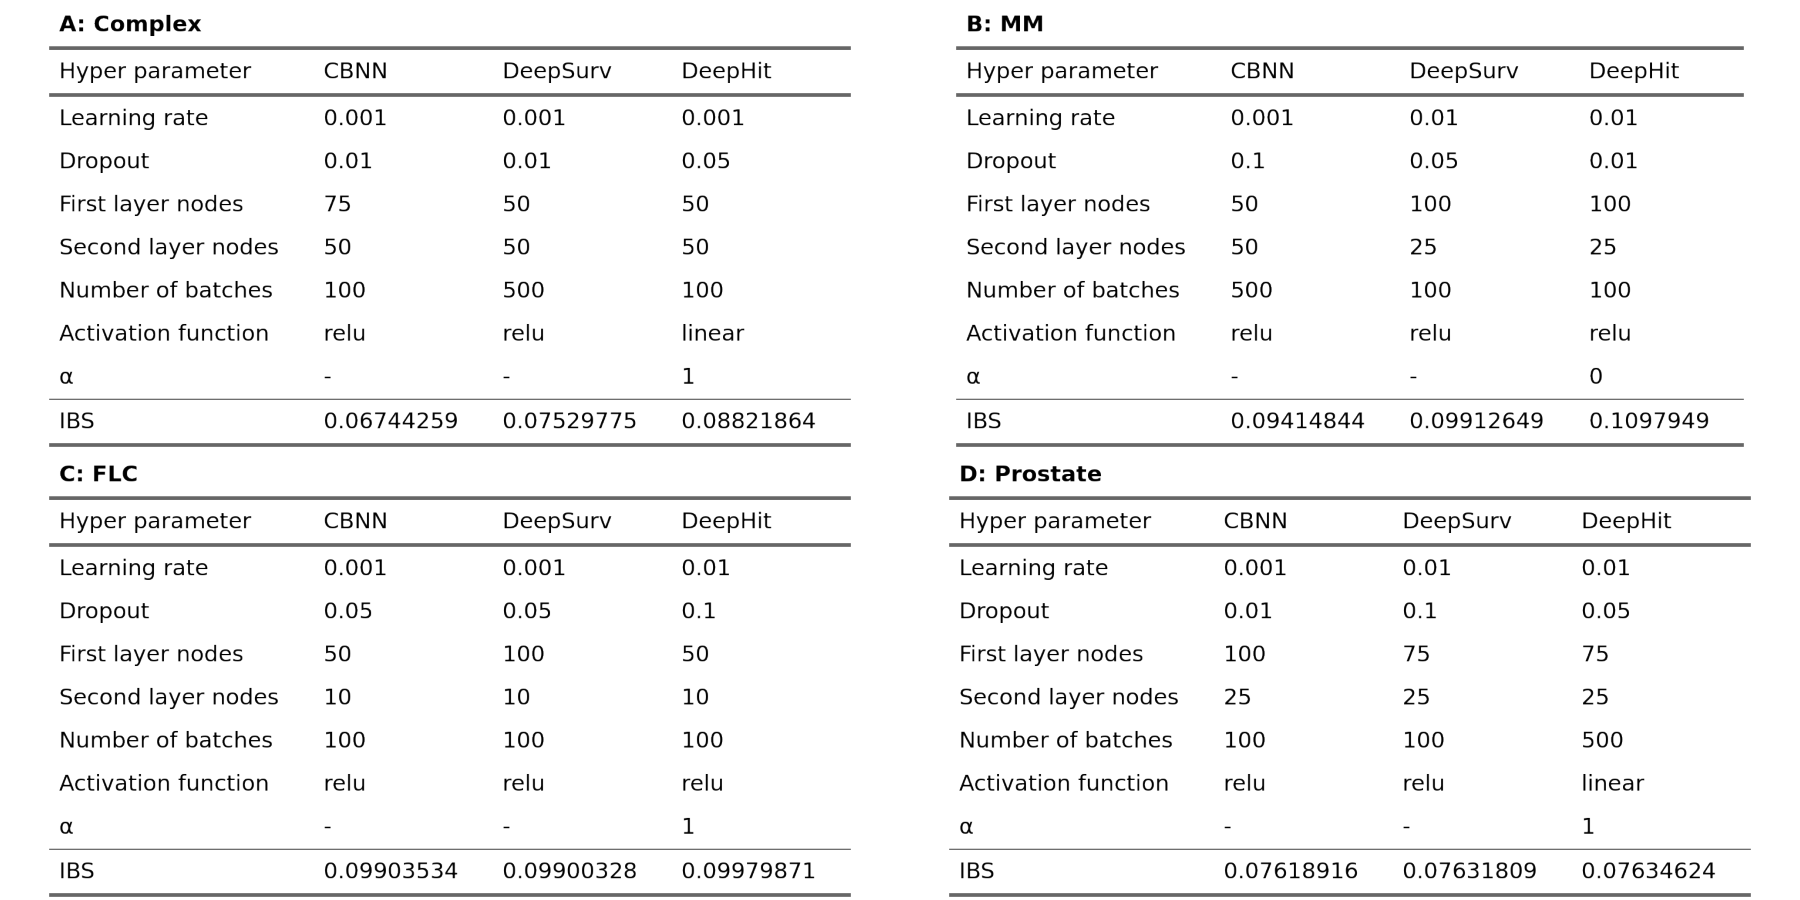
\includegraphics[width=1\linewidth]{../figures/Table1.pdf} \end{center}
\end{table}

DeepHit uses $\alpha$ as a hyperparameter, while DeepSurv and CBNN do not. We track IBS on the validation set for each hyperparameter combination,
choosing the combination with the lowest score for each method (Table \ref{tab:wins}).

\hypertarget{software-implementation}{%
\subsection{Software implementation}\label{software-implementation}}

R \citep{Rsoft} and Python \citep{py} are used to evaluate methods from both languages. We fit the Cox model using the \textbf{survival} package
\citep{survpkg} and the CBLR model using the \textbf{casebase} package \citep{cbpkg}. Both DeepSurv and DeepHit are fit using \textbf{pyCox}
\citep{lee2018DeepHit}. We made the components of CBNN using the \textbf{casebase} package \citep{cbpkg} for the sampling step and the
\textbf{keras} package \citep{keras} for our neural network architecture. We use the \textbf{simsurv} package \citep{simsurv} for our simulation studies
and \textbf{flexsurv} \citep{flexsurv} to fit a flexible baseline hazard using splines for our complex simulation. The \textbf{riskRegression} package
\citep{riskRegression} is used to get the IPA and $AUC_{IPCW}$. We modify the \textbf{riskRegression} package to be used with any user supplied
risk function \(F\). We use the \textbf{reticulate} package \citep{reticulate} to run both R based methods and Python based methods on the same seed.



%%%%%%%%%%%%%%%%%%%%%%%%%%%%%%%%%%%%%%%%%%%%%%
%%%%%%%%%%%%%%%%%%%%%%%%%%%%%%%%%%%%%%%%%%%%%%
%%%%%%%%section3
%%%%%%%%%%%%%%%%%%%%%%%%%%%%%%%%%%%%%%%%%%%%%%
%%%%%%%%%%%%%%%%%%%%%%%%%%%%%%%%%%%%%%%%%%%%%%



\begin{figure}

{\centering 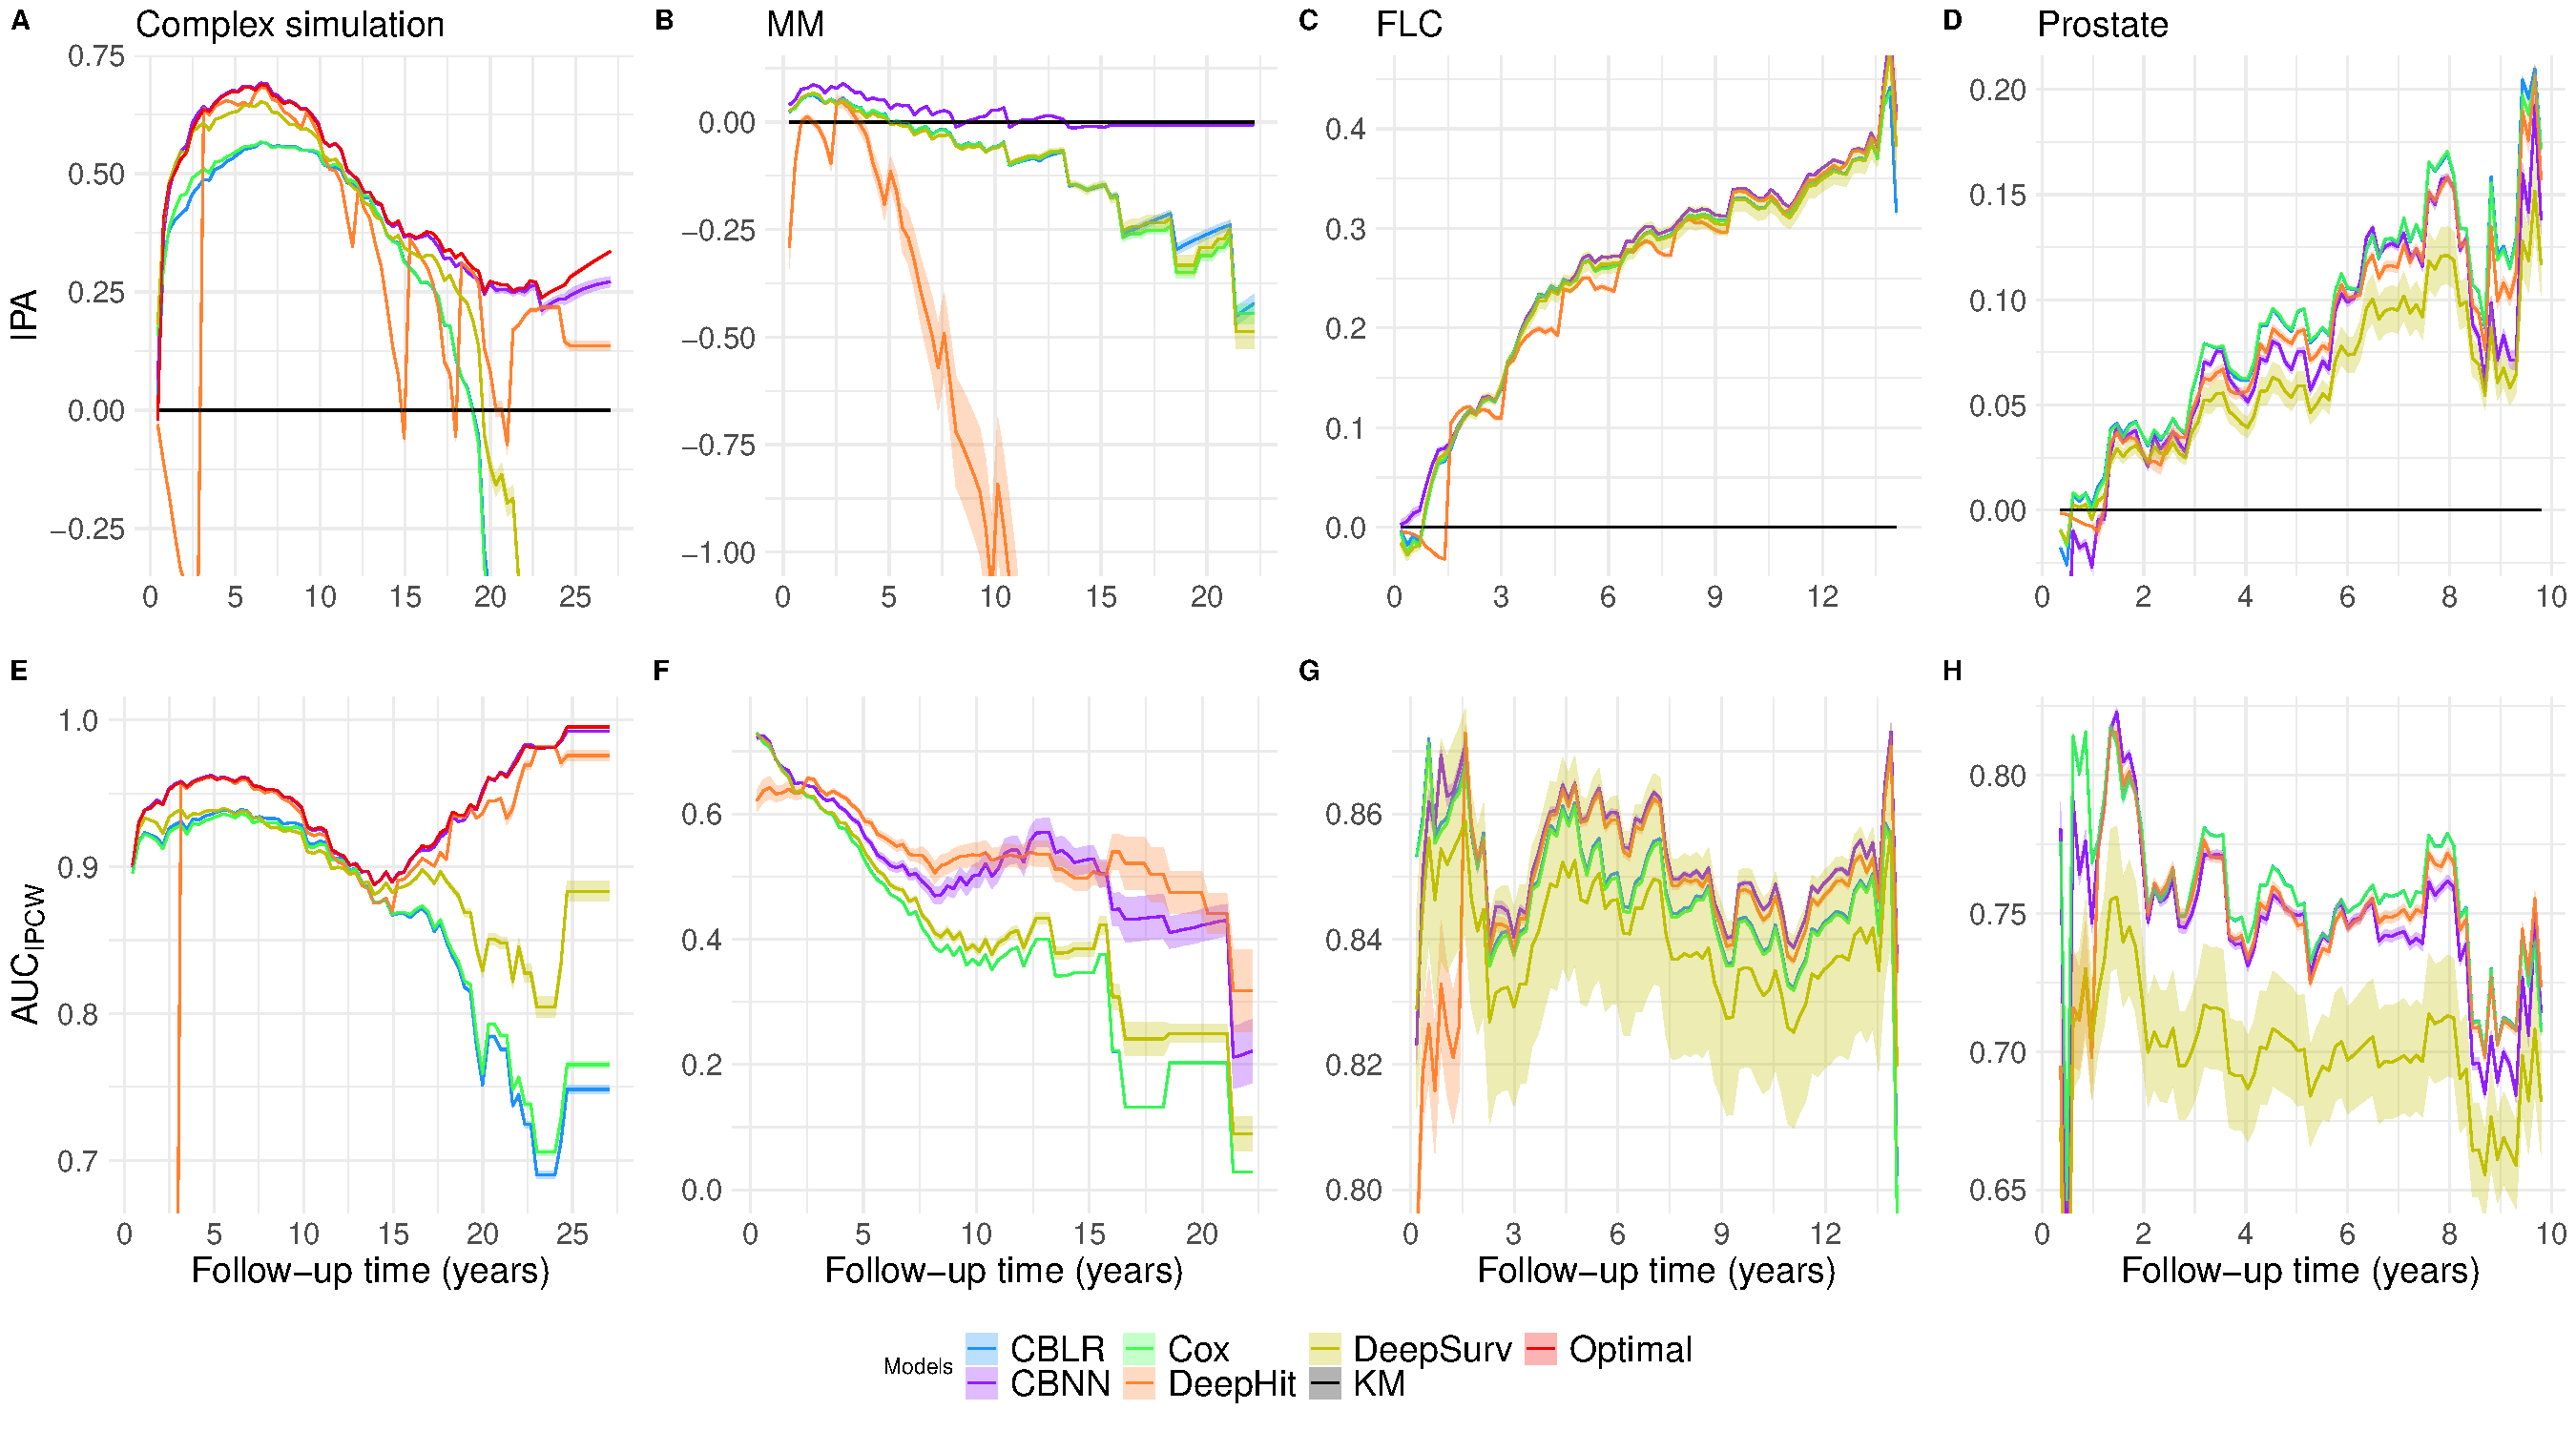
\includegraphics[width=1\linewidth]{../figures/Figure2.pdf} 

}

\caption{Performance of each model in the complex simulation (A, E), multiple myeloma (MM) case study (B, F), free light chain (FLC) case study (C, G)
and prostate cancer (Prostate) case study (D, H). The first row shows the IPA for each model in each study over follow-up time. Negative values mean
the model performs worse than the null model and positive values mean the model performs better. The second row shows the $AUC_{IPCW}$ for
each model in each study over follow-up time, where higher is better. Each model-specific metric in each study shows a 95\% confidence interval over 100 iterations. Metrics
are shown for six models: Case-Base with Logistic Regression (CBLR), Case-Base Neural Network (CBNN), Cox Proportional Hazard (Cox), DeepHit
and DeepSurv. The Kaplan-Meier (KM) model serves as a baseline, predicting the average curve for all individuals. CBLR and Cox have near identical
performance, resulting in curves that overlap. The Optimal model (a CBLR model with the exact interaction terms and baseline hazard specified) shows
the best performance we can expect on the simulated data.}\label{fig:megaPlot}
\end{figure}



\hypertarget{sims}{%
\section{Simulation study}\label{sims}}

We simulate data to evaluate the performance of CBNN in comparison with existing regression (Cox, CBLR) and neural network (DeepHit, DeepSurv)
methods. We specify a linear combination of each covariate as the linear predictor in the regression-based methods (Cox, CBLR), which contrasts
with neural network approaches that allow for approximations of non-linear interactions. The simulated data are based on a complex baseline hazard with time-varying
interactions, each with 10\% random censoring. We simulate three covariates for 5000 individuals:

\[
z_{1} \sim \textrm{Bernoulli}(0.5) \qquad \qquad %technically a control and treatment group
z_{2} \sim \begin{cases}
 N(0,0.5) & \textrm{if } z_{1}=0\\ 
 N(1,0.5) & \textrm{if } z_{1}=1
\end{cases} \qquad \qquad
z_{3} \sim N(1,0.5).
\]
In addition to the methods described above, we include the exact functional form of the covariates in a CBLR model (referred to as Optimal for simplicity)
in the complex simulation. We obtain confidence intervals by conducting 100 bootstrap re-samples on the training data. We keep 15\% of the data for testing before
hyperparameter selection. We use 15\% of the remaining data for validation and the rest is reserved for training. We predict risk functions for individuals in
the test set, which are used to calculate our IPA and $AUC_{IPCW}$. 





\hypertarget{complex-simulation-flexible-baseline-hazard-time-varying-interactions}{%
\subsection{Complex simulation: flexible baseline hazard, time-varying
interactions}\label{complex-simulation-flexible-baseline-hazard-time-varying-interactions}}

We use this simulation to assess performance on data with a complex baseline hazard and a time-varying interaction. We design the model \begin{align}
\log h(t \mid X_i) =\sum_{i=1}^{5} (\gamma_{i} \cdot \psi_{i}) + \beta_{{1}} (z_{1}) + \beta_{{2}} (z_{2})+ \beta_{{3}} (z_{3})+ \tau_{1} ( z_{1} \cdot t)+ \tau_{2} (z_{2} \cdot z_{3}), \nonumber
\end{align} where
\(\gamma_{1}=3.9, \gamma_{2}=3, \gamma_{3}=-0.43, \gamma_{4}=1.33,\gamma_{5}=-0.86, \beta_{{1}}=-5, \beta_{{2}}=-1, \beta_{{3}}=1, \tau_{1}=0.001, \tau_{2}=-1\)
and \(\psi_{i}\) are basis splines. The \(\gamma\) coefficients are obtained from an intercept-only cubic splines model with three knots using the \emph{flexsurvspline}
function from the \textbf{flexsurv} package \citep{flexsurv} on the German Breast Cancer Study Group dataset as it provides a complex baseline hazard from which
we can simulate. The study comprised 686 women with breast cancer followed between 1984 and 1989 \citep{royston2002flexible}. These $\gamma$, $\beta$ and $\tau$ coefficients are used
as our baseline hazard parameters and are fixed for the analysis. The \(\beta\) coefficients represent direct effects, \(\tau_{2}\) represents an interaction and
\(\tau_{1}\) is a time-varying interaction.

\hypertarget{performance-comparison-in-complex-simulation}{%
\subsection{Performance comparison in complex
simulation}\label{performance-comparison-in-complex-simulation}}


Figure \ref{fig:megaPlot} A, E and Table \ref{tab:megaTable} shows the performance over time on a test set. The Optimal model acts as a reference for ideal performance on the simulated data. For discrimination, the Optimal model performs best,
followed by CBNN, DeepHit, DeepSurv and the linear models (Figure \ref{fig:megaPlot} E). For both   To obtain a more realistic performance assessment, we compared
models in three case studies with a time-to-event outcome.


\begin{table}[!htbp]
\caption{Performance at certain percentages of follow-up time in the complex simulation (A), multiple myeloma (MM) case study (B), free light chain (FLC)
case study (C) and prostate cancer (Prostate) case study (D). Each table shows performance for each method in each study at $25\%$, $50\%$, $75\%$
and $100\%$ of follow-up time. These tables are included to
provide exact measures of performance. The models of interest are case-base with logistic regression (CBLR), Cox, Case-Base Neural Network (CBNN),
DeepHit, DeepSurv, and Optimal (in the complex simulation). The best score at each percent of follow-up time is highlighted in bold. If the average performance
is tied, then all tied values are highlighted.}
\label{tab:megaTable}

\begin{center}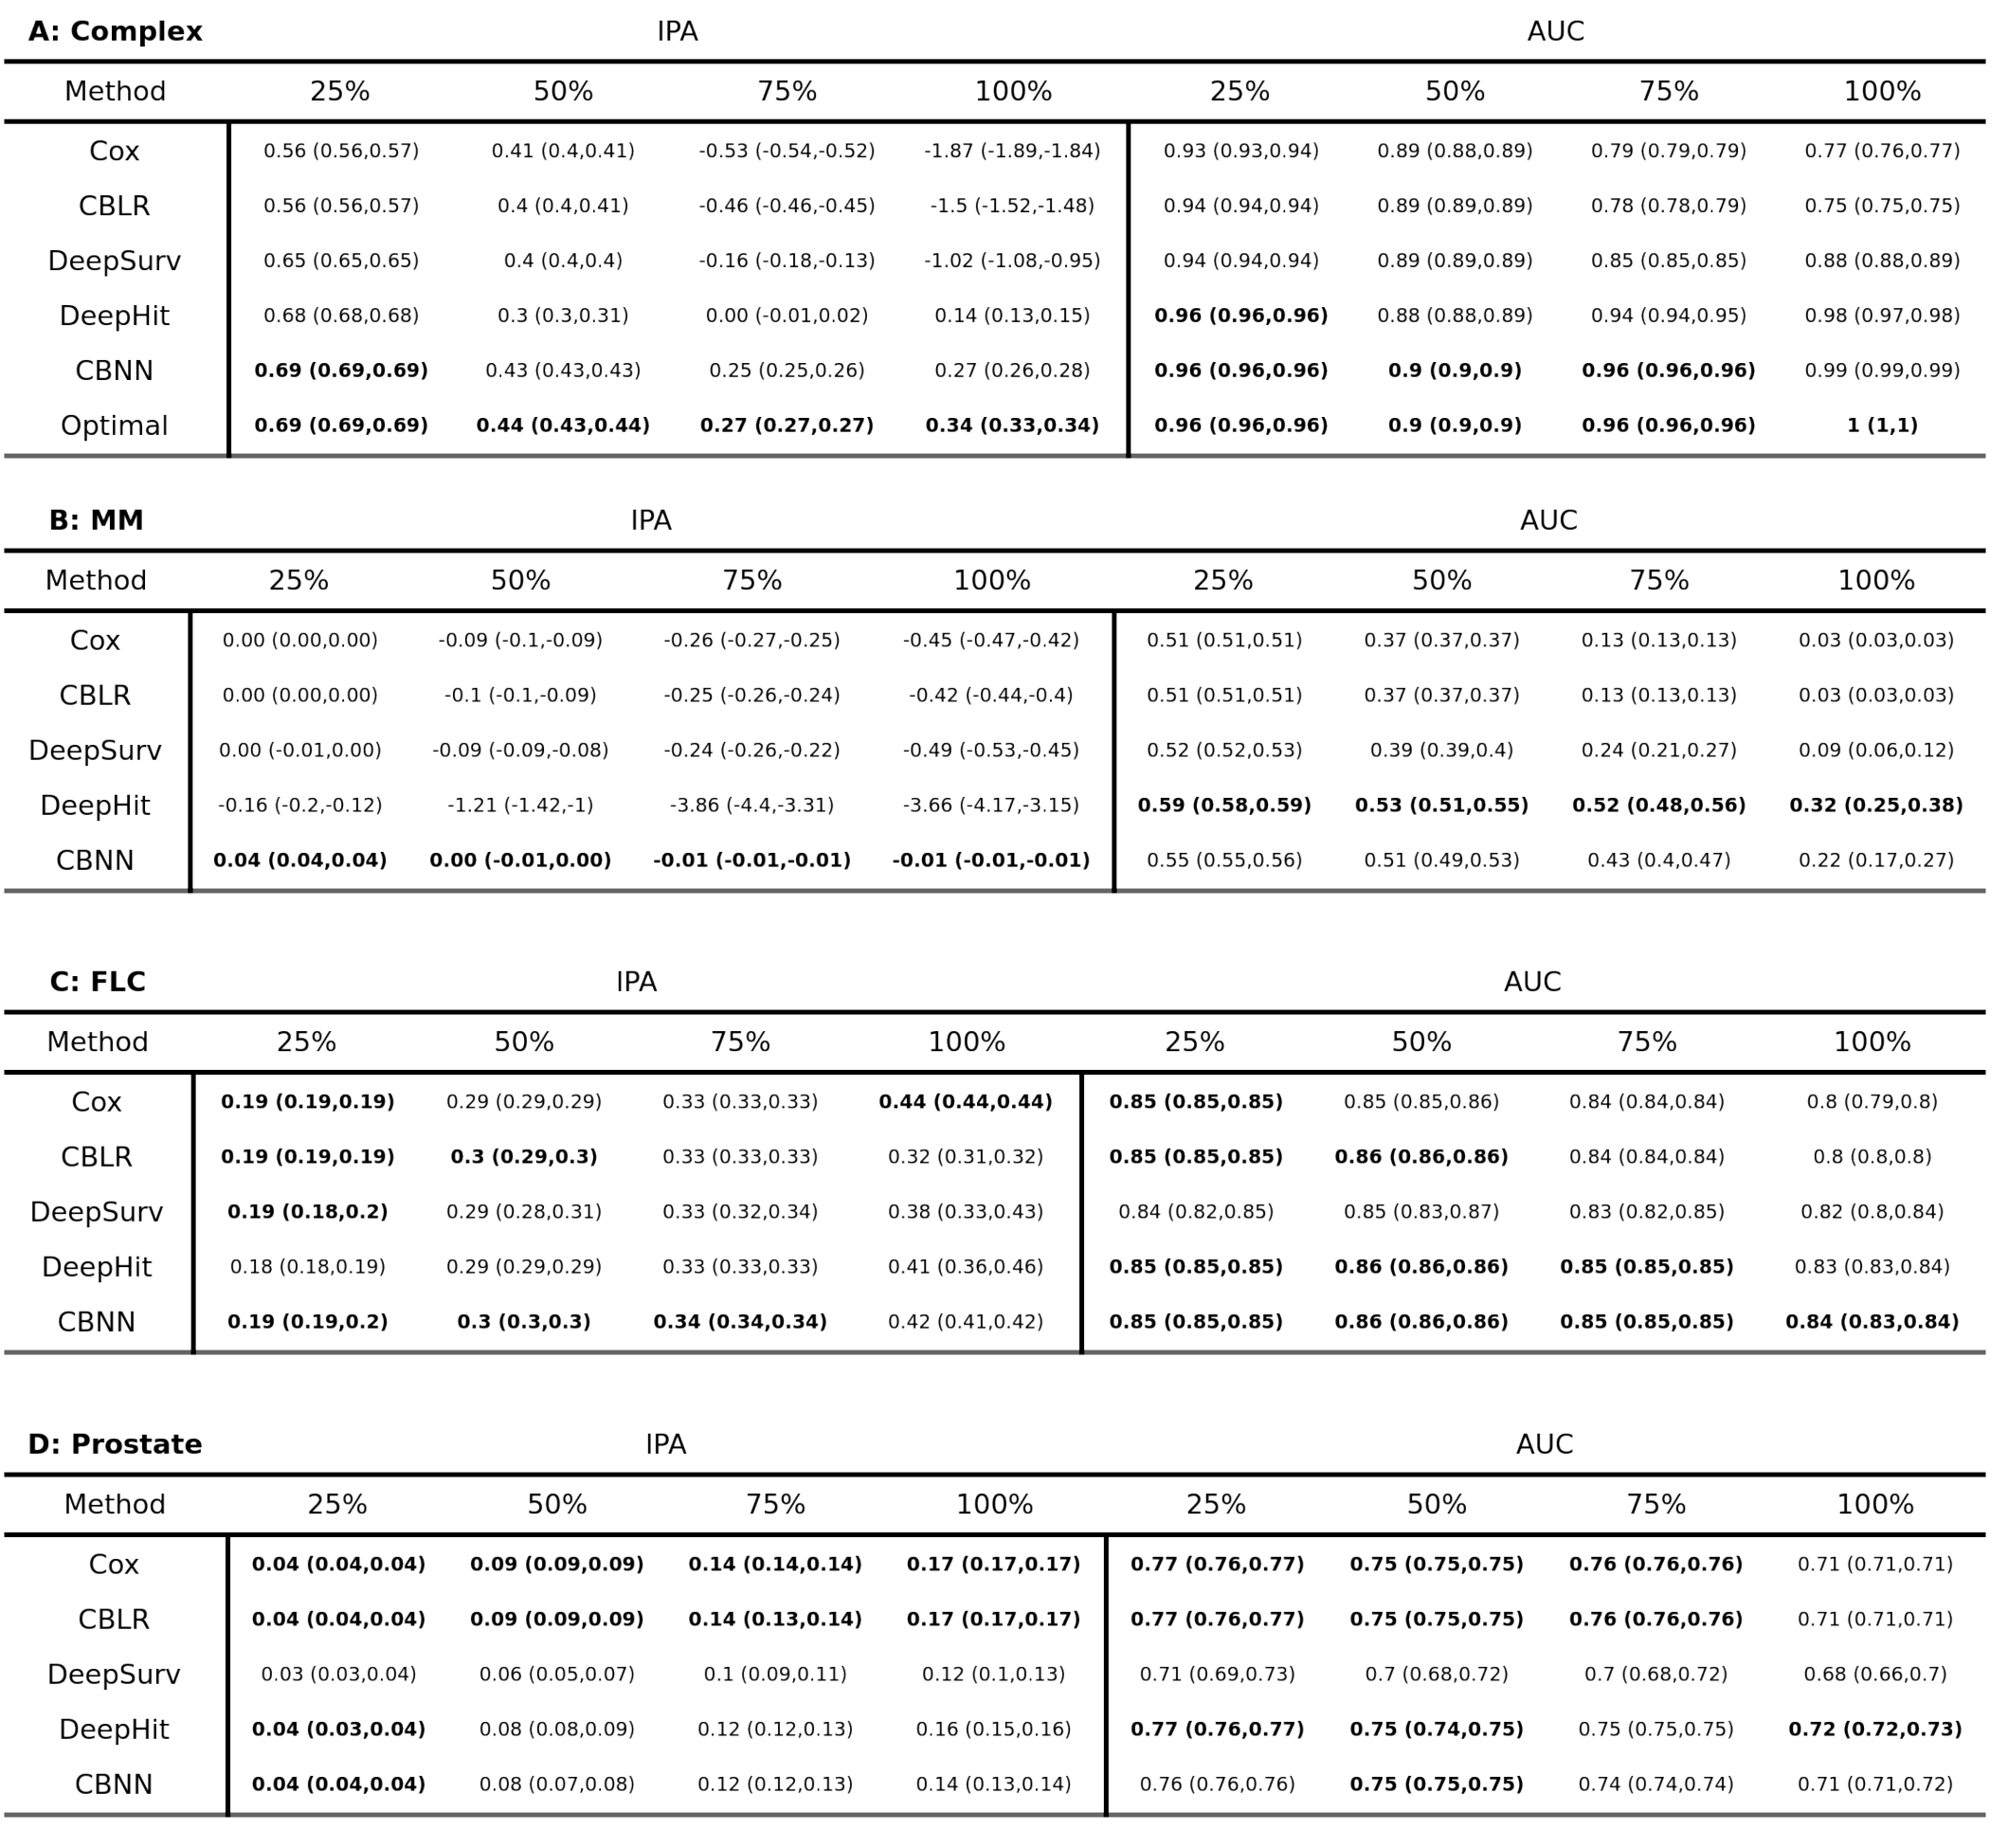
\includegraphics[width=1\linewidth]{../figures/Table2.pdf} \end{center}

\end{table}

%%%%%%%%%%%%%%%%%%%%%%%%%%%%%%%%%%%%%%%%%%%%%%
%%%%%%%%%%%%%%%%%%%%%%%%%%%%%%%%%%%%%%%%%%%%%%
%%%%%%%%section4
%%%%%%%%%%%%%%%%%%%%%%%%%%%%%%%%%%%%%%%%%%%%%%
%%%%%%%%%%%%%%%%%%%%%%%%%%%%%%%%%%%%%%%%%%%%%%


\hypertarget{casestudies}{%
\section{Case studies}\label{casestudies}}

The simulation examines whether a complex baseline hazard and time-varying interactions affect method performance.
The case study assesses performance in more realistic conditions, where we may not know if a flexible baseline hazard is beneficial, or if time-varying covariates
exist. For each dataset, we perform a grid search with the same hyperparameter procedure as described in the simulation (three-fold cross-validated grid search).
We then predict risk functions for everyone in the test set with the selected hyperparameters, which is used to calculate our metrics. We conduct 100-fold
bootstrap re-samples on the training data to get confidence intervals.

\hypertarget{pe-multiplemyeloma}{%
\subsection{Performance evaluation on multiple myeloma dataset}\label{pe-multiplemyeloma}}
We expect cancer may have risk factors that vary with time \citep{coradini2000time}. As such, the first case study examines multiple myeloma (MM),
using a cohort of 3882 patients seen at the Mayo Clinic from 1947 to 1996 until death \citep{myeloma}. Data are provided by the \textbf{survival} package \citep{survpkg}.
We use two covariates, year of entry into the study and the time of MM diagnosis \citep{myeloma}. We see 71\% incidence over 23 years \citep{myeloma}.

Figure \ref{fig:megaPlot} B, F and Table \ref{tab:megaTable} B demonstrate the performance over time on a test set. For discrimination, CBNN and DeepHit have a
similar performance, followed by DeepSurv and finally the linear models performing worst (Figure \ref{fig:megaPlot} F). For both discrimination and calibration, CBNN
performs substantially better than the linear models and DeepSurv, with DeepHit having the worst performance overall (Figure \ref{fig:megaPlot} B). Together, CBNN
is the best calibrated model and one of the best at discrimination in the MM case study.

%paragraph about performance

\hypertarget{pe-flc}{%
\subsection{Performance evaluation on free light chain dataset}\label{pe-flc}}
Serum free light chain (FLC) is a known diagnostic tool for assessing MM \citep{mm2flc}. We are interested in whether there is a predictive benefit if the FLC markers
varies with time. As such the second case study examines the relationship between serum FLC and mortality in a random sample of half the individuals in
$\frac{2}{3}$ of the residents of Olmsted County over the age of 50 \citep{flc}. Data are provided by the \textbf{survival} package \citep{survpkg} for 7874 subjects tracked
until death with 27\% incidence over 14 years \citep{flc}. We use five covariates, total serum FLC (sum of kappa and lambda), age, sex, serum creatine and monoclonal gammopathy state \citep{flc}.

Figure \ref{fig:megaPlot} C, G and Table \ref{tab:megaTable} C demonstrate the performance over time on a test set. CBNN, DeepHit and the linear models perform best at
discrimination, followed by DeepSurv (Figure \ref{fig:megaPlot} G). The rankings remain the same aside from DeepHit where the performance periodically drops to worse
than DeepSurv (Figure \ref{fig:megaPlot} C). Together, CBNN outperforms the competing models in terms of both calibration and discrimination.
However, CBNN is only slightly better than the linear ones.

\hypertarget{pe-prostate}{%
\subsection{Performance evaluation on prostate cancer dataset}\label{pe-prostate}}
As the CBNN model saw large predictive benefits on MM and small predictive benefits on FLC, we wish to examine longitudinal data with a more complex risk profile.
The third case study (Prostate) examines prostate cancer survival on a publicly available simulation of the Surveillance, Epidemiology, and End Results (SEER) medicare study \citep{prostate}.
The Prostate dataset, which is contained in the \textbf{asaur} package \citep{asaur}, has a record of competing risks. As we are only interested in the single event scenario,
we only keep individuals with prostate cancer death or censoring. This subset tracks 11054 individuals with three covariates: differentiation grade, age group and cancer
state. There is a 7\% incidence over 10 years \citep{prostate}.

Figure \ref{fig:megaPlot} C, G and Table \ref{tab:megaTable} C demonstrate the performance over time on a test set. In the prostate case study, the linear models outperform the other
models in both discrimination and calibration, followed by CBNN and DeepHit and finally DeepSurv (Figure \ref{fig:megaPlot} C, G). Aside from DeepSurv, the performance is
similar across all models.



%%%%%%%%%%%%%%%%%%%%%%%%%%%%%%%%%%%%%%%%%%%%%%
%%%%%%%%%%%%%%%%%%%%%%%%%%%%%%%%%%%%%%%%%%%%%%
%%%%%%%%section6
%%%%%%%%%%%%%%%%%%%%%%%%%%%%%%%%%%%%%%%%%%%%%%
%%%%%%%%%%%%%%%%%%%%%%%%%%%%%%%%%%%%%%%%%%%%%%


\hypertarget{discussion}{%
\section{Discussion}\label{discussion}}

CBNNs model survival outcomes by using neural networks on case-base sampled data. We incorporate follow-up time as a feature, providing a data-driven
estimate of a flexible baseline hazard and time-varying interactions in our hazard function. The two competing neural network models we evaluated cannot
model time-varying interactions \citep{katzman2018DeepSurv} \citep{lee2018DeepHit}. The CBNN model performs better due to its ability to model time-varying
interactions and a complex baseline hazard.

The complex simulation requires a method that can learn both time-varying interactions and have a flexible baseline hazard. Based on our complex simulation results (Figure \ref{fig:megaPlot} A, E and Table \ref{tab:megaTable} A), CBNN
outperforms the competitors. This simulation shows how all models perform under ideal conditions with minimal noise in the data, while the three
case studies assess their performance in realistic conditions. In the MM case study, flexibility in both interaction modeling and baseline hazard
improves the performance of CBNN over the other models, suggesting that this flexibility aids calibration (Figure \ref{fig:megaPlot} B, F and Table
\ref{tab:megaTable} B). Upon examination of the FLC case study, CBNN demonstrates a small improvement to performance compared to the linear
models and DeepHit for both IPA and AUC (Figure \ref{fig:megaPlot} C, G and Table \ref{tab:megaTable} C). In the Prostate case study, the linear
models outperform the neural network ones, while CBNN and DeepHit alternate their positions depending on the follow-up time of interest and DeepSurv
maintains last place (Figure \ref{fig:megaPlot} C, G and Table \ref{tab:megaTable} C). We attribute this to potential over-parameterization in the neural
network models, as we did not test for fewer nodes in each hidden layer, even with dropout. Though the ranking places the linear models above the
neural network ones, their overall performance falls within a small range of IPA and AUC values aside from DeepSurv.

Compared to CBNN, the neural network competitors also have limitations. DeepSurv is a proportional hazards model and does not estimate the baseline
hazard \citep{katzman2018DeepSurv}. DeepHit requires an alpha hyperparameter, assumes a single distribution for the baseline hazard and models the
survival function directly \citep{lee2018DeepHit}. The alternative neural network methods match on time, while CBNN models time directly. Another method
caught our interest during our literature review. Deep Survival Machines (DSM), a parametric survival model using neural networks with a mixture of
distributions that can fit a flexible baseline hazard \citep{dsmPaper}. With our hyperparameter options, DSM did not converge in the complex
simulation which may have been due to issues in software or method specific limitations. Therefore, we did not include this method in our comparison.

While we apply a full grid search with three-fold cross-validation for all neural network models, there are an infinite number of untested hyperparameters we did not test. A completely
exhaustive search is computationally infeasible, therefore it is reasonable to expect that there is a set of hyperparameters that is better suited for each model
in each study. However, we test a reasonably large range while accounting for potential over-fitting by including dropout \citep{gulli2017}. We provide the same
options to all models aside from DeepHit, which has a method specific hyperparameter $\alpha$ \citep{lee2018DeepHit}. With these limitations in mind, we
summarize the differences in performance across all tested methods.

If prediction is our goal, we suggest CBNN as the best model in the Complex simulation, MM case study and FLC case study. The linear models were
competitive in the FLC case study and performed best in the Prostate case study. Though neural network interpretability is steadily improving \citep{interpret},
there is still a trade-off compared to regression models, especially when the predictive performance gain is minimal, like in the FLC case study. We suggest
that reference models should be included when assessing neural network models. Both a null model (KM curve) and a linear model (either Cox or a flexible
baseline hazard model like CBLR) provide insight as to whether the neural network model is learning anything useful beyond linear predictors that were
not accounted for.

\section{Conclusions}\label{sec5}

Our study was motivated by the lack of easily implemented survival models based on neural networks that can approximate time-varying interactions.
This lead us to repurpose the case-base sampling technique, which has previously been used with logistic regression \citep{hanley2009}, to neural network models for a data driven
approach to time-varying interaction modeling. In our paper, We aim to compare CBNNs with existing methods. We assess the discrimination and calibration
of each method in a simulation with time-varying interactions and a complex baseline hazard, and three case studies. CBNNs outperform all competitors in
the complex simulation and two case studies while maintaining competitive performance in a final case study. Once we perform case-base sampling and
adjust for the sampling bias, we can use a sigmoid activation function to predict our hazard function. Our approach provides an alternative to incorporating
censored individuals, treating survival outcomes as binary ones. Forgoing the requirement of custom loss functions, CBNNs only require the use of standard
components in machine learning libraries (specifically, the add layer to adjust for sampling bias and the sigmoid activation function) after case-base sampling.
Due to the simplicity in its implementation and by extension user experience, CBNNs are both a user-friendly approach to data-driven, single event survival analysis and is
easily extendable to any feed-forward neural network framework.

%\backmatter

\hypertarget{data-and-code-availability-statement}{%
\subsection*{Data and code availability
statement}\label{data-and-code-availability-statement}}
\addcontentsline{toc}{section}{Data and code availability statement}


The MM and FLC datasets are available in the \textbf{survival} package in R
\citep{survpkg}. The Prostate dataset is available as part of the \textbf{asaur} package in R \citep{asaur}.
The code for this manuscript and its analyses can be found at \url{https://github.com/Jesse-Islam/cbnnManuscript}. The software package making CBNN
easier to implement can be found at \url{https://github.com/Jesse-Islam/cbnn}.

\hypertarget{acknowledgements}{%
\subsection*{Acknowledgements}\label{acknowledgements}}
\addcontentsline{toc}{section}{Acknowledgements}

We would like to thank Dr.~James Meigs, the project leader of UM1DK078616 and R01HL151855, for his support and helpful discussions.
We would also like to thank Dr.~James Hanley for his support and discussions while extending the case-base methodology.

\subsection*{Author contributions}

J.I. conceived the proof of concept, developed the theoretical formalism, developed the neural network code base,
wrote the majority of the manuscript and performed the simulations and analyses. M.T. wrote the majority of the case-base sampling section \ref{case-base-sampling}.
M.T. and S.B. provided key insights into the core sampling technique (case-base). R.S. provided multiple edits to the manuscript structure and key insights. All authors
discussed the results and contributed to the final manuscript.

\subsection*{Financial disclosure}

This work was supported by subcontracts from UM1DK078616 and R01HL151855
to R.S. The work was also supported as part of the Congressionally Directed Medical Research Programs (CDMRP) award W81XWH-17-1-0347.
\subsection*{Conflict of interest}

The authors declare no potential conflict of interests.


\appendix
%\nocite{*}% Show all bib entries - both cited and uncited; comment this line to view only cited bib entries;
\bibliography{CBNNManuscript}%

\end{document}
